%% Autor: Björn Ritterbecks 
%% Letzte Aenderung: 15.06.2016 
\thisfloatsetup{%
  capbesidewidth=\marginparwidth}
\begin{figure}[htbp]
\vspace*{0.2cm}
\centering
%\sansmath
 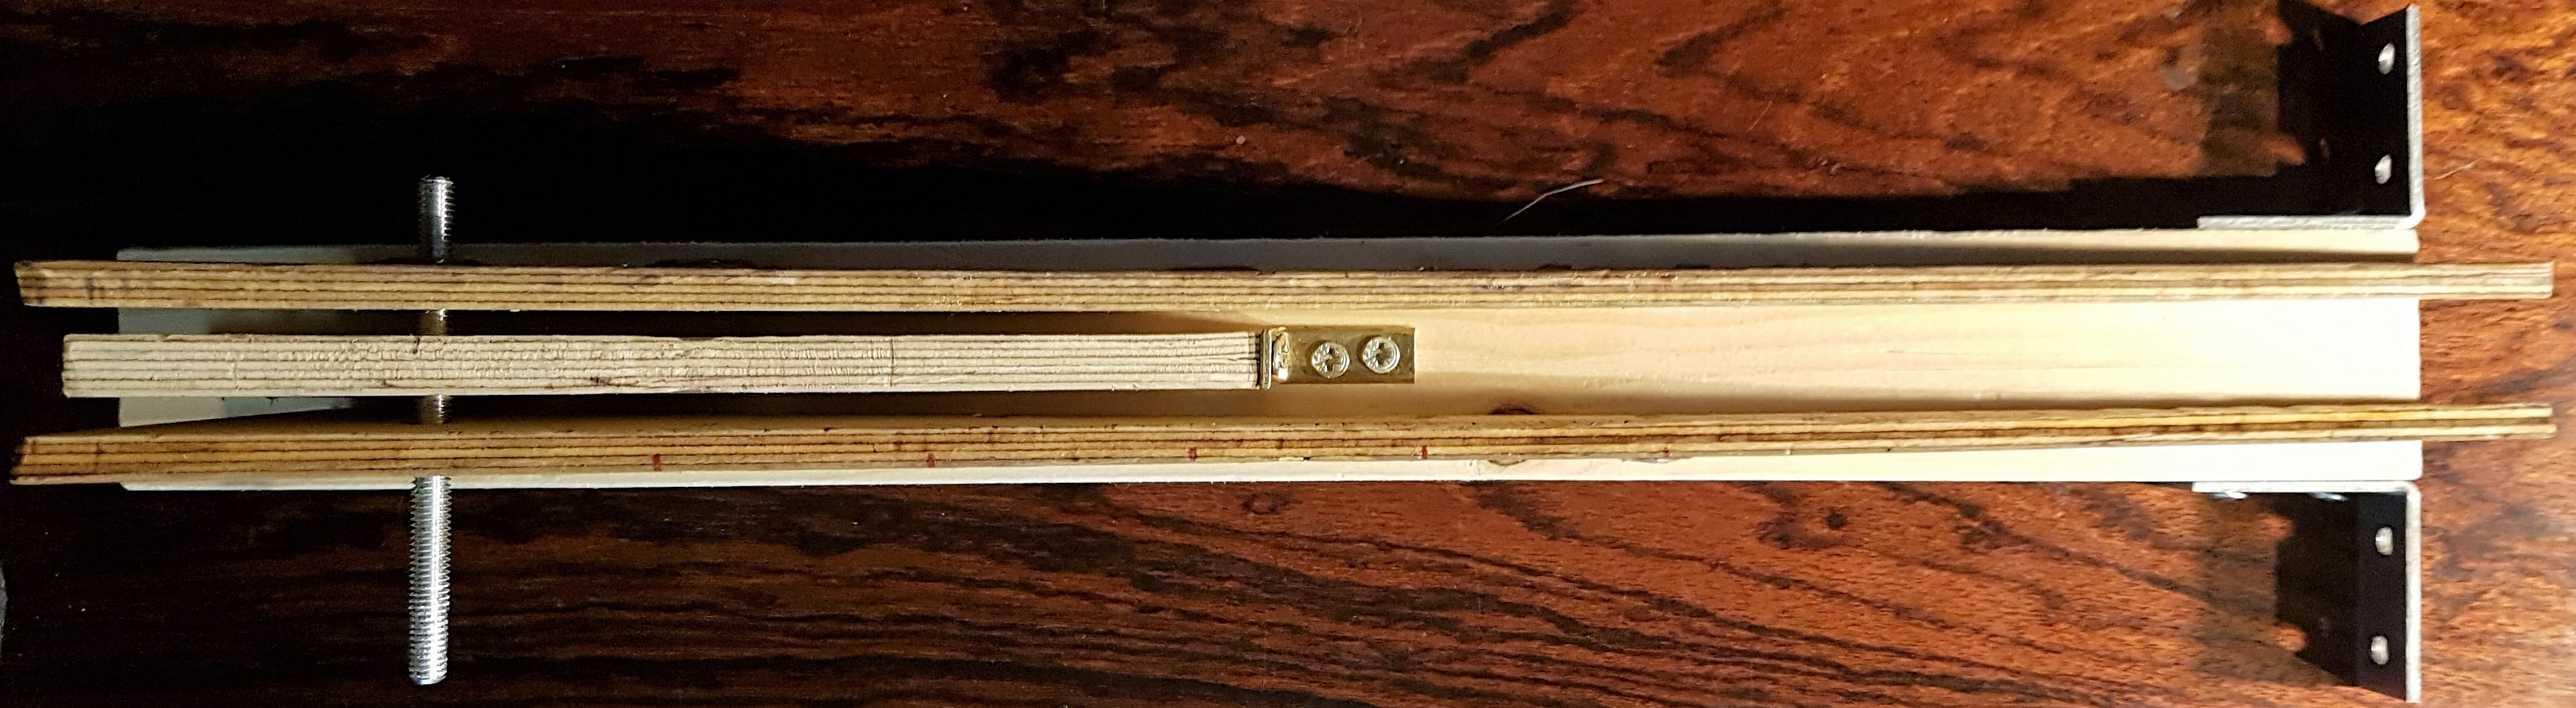
\includegraphics[width=0.99\textwidth]{images/rrampe1.jpg}
  \caption[Draufsicht der gebauten Rampe]{Die Startrampe ist auf ein Brett montiert, welches wiederum mit zwei Winkeln an den Experimentiertisch angeschraubt werden kann. Durch die Anordnung auf einem schmalen Brett lässt sich zum Einen die Rechtwinkligkeit gut überprüfen, zum Anderen erlaubt es den Zahnrädern in vertikaler Richtung bis unterhalb der Tischplatte zu reichen. Auf der linken Seite mittig ist ein Holzblock mit Ausbohrungen, durch welche die Gewindestangen zur Zentrierung gesteckt hätten werden sollen.}
  \label{fig:rampfenschliff2}
  \vspace{-0pt}
\end{figure}